Trên cơ sở phân tích và đánh giá các giải pháp hỗ trợ du lịch hiện có ở Chương 4, chương này đề xuất Hệ thống Gợi ý Hành trình Du lịch Thông minh TravelEZ nhằm giải quyết các hạn chế đã được chỉ ra. Hệ thống được cấu thành từ các nhóm chức năng chính, mỗi nhóm đảm nhiệm một vai trò chuyên biệt để hiện thực hóa mục tiêu xây dựng một nền tảng du lịch toàn diện — từ việc tạo ra các gợi ý cá nhân hóa sâu sắc, thúc đẩy tương tác cộng đồng, cho đến việc cung cấp công cụ hỗ trợ cho các nhà cung cấp dịch vụ.

Hệ thống bao gồm 8 module chính sau:

% --- HÌNH ẢNH TỔNG QUAN ĐƯỢC ĐẶT NGAY TRƯỚC DANH SÁCH MODULE ---
\begin{figure}[H]
    \centering
    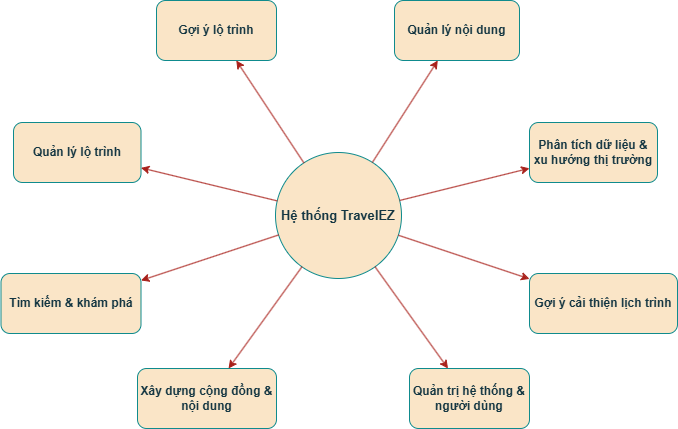
\includegraphics[width=0.9\textwidth]{Images/5 Hệ thống đề xuất/System Overview.png} 
    \caption{Sơ đồ tổng quan các thành phần chính của hệ thống TravelEZ.}
    \label{fig:system_overview}
\end{figure}

% --- MÔ TẢ CHI TIẾT CÁC MODULE ---
\begin{enumerate}
    \item \textbf{MD-01 Gợi ý lộ trình:} Tiếp nhận yêu cầu lập kế hoạch (điểm đến, thời gian, ngân sách, sở thích), xử lý và đề xuất kế hoạch lộ trình chi tiết (theo ngày/khung giờ). Người dùng tùy chỉnh lộ trình (thêm/xoá/sắp xếp lại điểm đến, điều chỉnh thời gian), lưu trữ và quản lý các phiên bản kế hoạch.

    \item \textbf{MD-02 Quản lý lộ trình:} Người dùng có thể chia sẻ kế hoạch với bạn bè và tích hợp lộ trình với Google Calendar.

    \item \textbf{MD-03 Tìm kiếm và khám phá:} Cung cấp chức năng tìm kiếm thông tin (địa điểm, dịch vụ, bài viết), lọc kết quả nâng cao (khu vực, loại hình, đánh giá, độ phổ biến), hiển thị kết quả trên bản đồ tương tác, lưu (bookmark) nội dung yêu thích vào bộ sưu tập cá nhân. 

    \item \textbf{MD-04 Xây dựng cộng đồng và nội dung:} Cho phép đăng tải bài viết, đánh giá (review) và xếp hạng (rating) cho dịch vụ, tương tác (bình luận, theo dõi), quản lý hồ sơ cá nhân và các nội dung đã đóng góp.
    
    \item \textbf{MD-05 Quản lý nội dung:} Cung cấp giao diện cho quản trị viên quản lý nội dung đăng tải, kiểm duyệt, xử lý tài khoản vi phạm, tiếp nhận và xử lý báo cáo (report) từ người dùng.

    \item \textbf{MD-06 Phân tích dữ liệu và xu hướng thị trường:} Cung cấp dashboard (cho nhà cung cấp) hiển thị các số liệu thống kê, trực quan hóa dữ liệu và trình bày các xu hướng thịnh hành (điểm đến, chủ đề tìm kiếm).

    \item \textbf{MD-07 Gợi ý cải thiện lịch trình:} Phân tích các lộ trình/tour hiện có của nhà cung cấp dịch vụ, cung cấp các gợi ý điều chỉnh cụ thể.

    \item \textbf{MD-08 Quản trị hệ thống \& người dùng:} Xử lý xác thực người dùng, quản lý hồ sơ người dùng, phân quyền truy cập (admin, provider, tourist), quản
    
\end{enumerate}
